\section{Modellazione}

\subsection{Modelli notevoli}

\begin{multicols}{2}

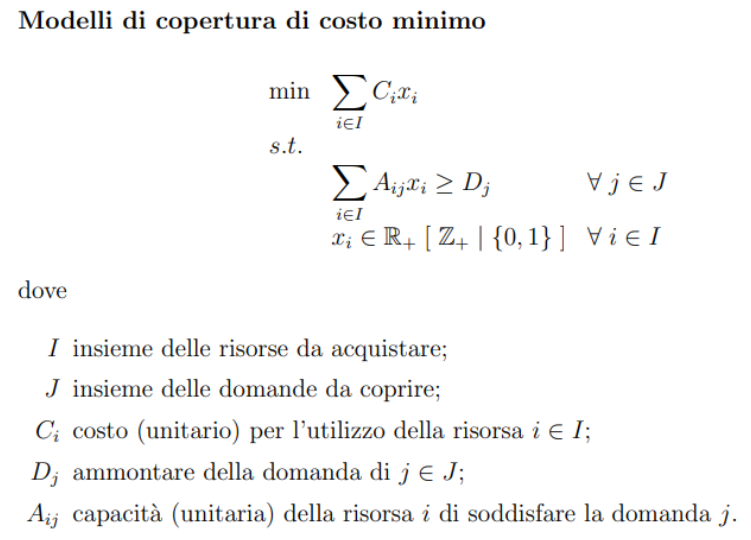
\includegraphics[width=\linewidth]{img/copertura-costo-minimo.png}
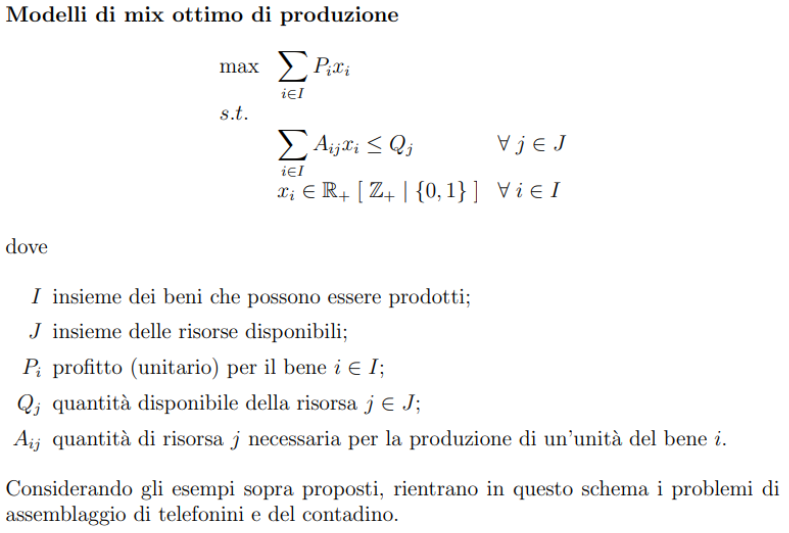
\includegraphics[width=\linewidth]{img/mix-ottimo.png}
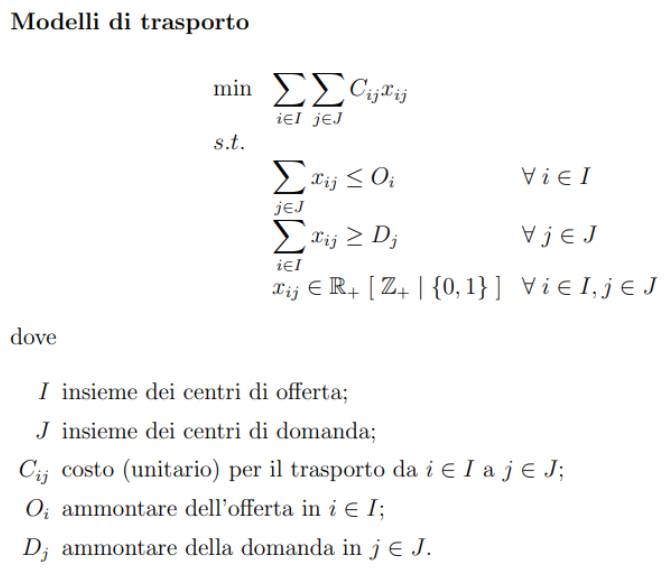
\includegraphics[width=\linewidth]{img/trasporti.png}
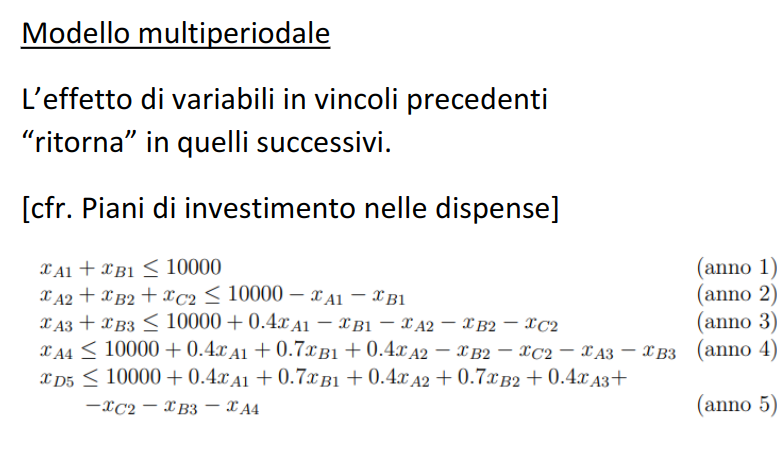
\includegraphics[width=\linewidth]{img/multiperiodale.png}

\end{multicols}
\subsection{Passaggi}
\begin{enumerate}
    \item Individuare le variabili decisionali;
    \item definire la funzione obiettivo;
    \item iniziare a stendere i vincoli non nella parte dei "tenendo conto che:";
    \item iniziare a stendere almeno un vincolo dell'elenco puntato che propone il professore\pro{Almeno uno o due di questi vincoli sono comodi per scrivere il resto del modello};
    \item Scrivere il resto dei vincoli.
\end{enumerate}

\subsubsection{Individuazione delle variabili decisionali}
Queste variabili sono solitamente a uno o due indici\gab{Spesso le variabii a due indici fanno danni, meglio mettere più variabili ad un indice se possibile.}.
Diventa invece preferibile mettere a due indice quando è evidente dal problema che servono entrambe due colonne di una tabella\footnote{Nel problema dei trasporti solitamente usiamo due indici.}.

Un'altra cosa a cui fare attenzione è la scrittura dei vincoli in cui un \textit{"Indipendentemente da"} ci fa capire che probabilmente avremo bisogno di una variabile ad un indice solo e non due.

\subsubsection{Definizione della funzione obiettivo}
La funzione obiettivo \textbf{DEVE} essere lineare\footnote{Se non è lineare, allora non è un problema di programmazione lineare. (detto più brevemente anche problema di PL).}.

É importante fare molta attenzione a non moltiplicare due variabili, anche se una delle due variabili è binaria.

\subsubsection{Vincoli}

Anche i vincoli \textbf{DEVONO} essere lineari.


